\section{Eigenstates of the Hamiltonian}

%
\subsection{The $\{\varphi_n\}$ representation}
Since none of the eigenvalues of $N$ ($H$) is degenerate, $N$ ($H$) alon constitutes a CSCO in $\E_c$.
%
\subsubsection{The basis vectors in terms of $\ket{\psi_0}$}
We assume that the vector $\ket{\varphi_0}$ which satsfies $a\ket{\varphi_0}=0$, is normalized. According to lemma III, the vector $\ket{\varphi_1}$ is proportional 
to $a^\dagger\ket{\varphi_0}$ in the form 
\begin{align*}
    \ket{\varphi_1}=c_1a^\dagger\ket{\varphi_0}.
\end{align*} 
We shall determine $c_1$ by requiring $\ket{\varphi_1}$ to e normalized and choosing the phase of $\ket{\varphi_1}$ such that $c_1$ is real and positive.
The square of the norm of $\ket{\varphi_1}$ is 
\begin{align*}
    \braket{\varphi_1|\varphi_1}=|c_1|^2\braket{\varphi_0|aa^\dagger|\varphi_0}=|c_1|^2\braket{\varphi_0|(a^\dagger a+1)|\varphi_0}=|c_1|^2[\underbrace{\braket{\varphi_0|N|\varphi_0}}_{0\braket{\varphi_0|\varphi_0}}+\braket{\varphi_0|\varphi_0}]=|C_1|^2.
\end{align*}
We find that $c_1=1$:
\begin{align}
    \braket{\varphi_1|\varphi_1}=|c_1|^2=1\Longrightarrow \ket{\varphi_1}=a^\dagger\ket{\varphi_0}.
\end{align}
We can do the same to constrcut $\ket{\varphi_2}$ from $\ket{\varphi_1}$ and get $c_2$ and so on. In general, if we know $\ket{\varphi_{n-1}}$ (normalized), then the 
normalized vector $\ket{\varphi_n}$ is written 
\begin{align*}
    \ket{\varphi_n}=c_na^\dagger\ket{\varphi_{n-1}},\quad\text{so that}\quad c_n=\frac{1}{\sqrt{n}}.
\end{align*}
In fact, we can express all $\ket{\varphi_n}$ in terms of $\ket{\varphi_0}$ by recursion:
\begin{align}
    \text{Excited states in terms of the ground state}\qquad\highlight{\ket{\varphi_n}=\frac{1}{\sqrt{n}}(a^\dagger)^n\ket{\varphi_0}}.
    \label{eq:excitedstatesfromground}
\end{align}
%
\subsubsection{Orthonormalization and closure relations}
Since $H$ is Hermitian, the kets $\ket{\varphi_n}$ corresponding to different values of $n$ are orthogonal so that they satisfy the orthonormalization relation:
\begin{align*}
    \braket{\varphi_n'|\varphi_n}=\delta_{nn'}.
\end{align*}
In addition, $H$ is an obsrvable; the set of the $\ket{\varphi_n}$ therefore constitutes a basis in $\E_x$, which is expressed by the closure relation
\begin{align*}
    \sum_n\ket{\varphi_n}\bra{\varphi_n}=\mathds{1}.
\end{align*}

%
\subsubsection{Action of the various operators}
The observables $X$ and $P$ are linear combinations of the operators $a$ and $a^\dagger$. Therefore, all physical quantities can be expressed in terms of the latters.
The action of $a$ and $a^\dagger$ on the vectors of the $\{\ket{\varphi_n}\}$ basis is 
\begin{align}
    \text{Action of $a$ and $a^\dagger$}\qquad
    \highlight{
    \begin{array}{l}
    a^\dagger\ket{\varphi_n}=\sqrt{n+1}\ket{\varphi_{n+1}}\\
    a\ket{\varphi_n}=\sqrt{n}\ket{\varphi_{n-1}}\end{array}\stackrel{\text{Adjoint}}{\longrightarrow}
    \begin{array}{l}
    \bra{\varphi_n}a=\sqrt{n+1}\bra{\varphi_{n+1}}\\
    \bra{\varphi_n}a^\dagger=\sqrt{n}\bra{\varphi_{n-1}} 
    \end{array}}
    \label{eq:actionofaa}
\end{align}
Note that $a$ decreases or increases $n$ by one unit depending on wheter it acts on the $\ket{\varphi_n}$ or on the bra $\bra{\varphi_n}$, similarly for $a^\dagger$.
The expressions for $X$ and $P$ are then:
\begin{align}
    X\ket{\varphi_n}=\sqrt{\frac{\hbar}{m\omega}}\frac{1}{\sqrt{2}}(a^\dagger+a)\ket{\varphi_n}=\sqrt{\frac{\hbar}{2m\omega}}[\sqrt{n+1}\ket{\varphi_{n+1}}+\sqrt{n}\ket{\varphi_{n-1}}]\\
    P\ket{\varphi_n}=\sqrt{m\hbar\omega}\frac{i}{\sqrt{2}}(a^\dagger-a)\ket{\varphi_n}=i\sqrt{\frac{m\hbar\omega}{2}}[\sqrt{n+1}\ket{\varphi_{n+1}}-\sqrt{n}\ket{\varphi_{n-1}}]
    \label{eq:XPintermsofaa}
\end{align}
The matrix elements of $a,a^\dagger,X,P$ in the $\{\ket{\varphi_n}\}$ representation are therefore
\begin{align}
    \braket{\varphi_{n'}|a|\varphi_n}=\sqrt{n}\delta_{n',n-1}\\
    \braket{\varphi_{n'}|a^\dagger|\varphi_n}=\sqrt{n+1}\delta_{n',n+1}\\
    \braket{\varphi_{n'}|X|\varphi_n}=\sqrt{\frac{\hbar}{2m\omega}}[\sqrt{n+1}\delta_{n',n+1}+\sqrt{n}\delta_{n',n-1}]\\
    \braket{\varphi_{n'}|P|\varphi_n}=i\sqrt{\frac{m\hbar\omega}{2}}[\sqrt{n+1}\delta_{n',n+1}-\sqrt{n}\delta_{n',n-1}]
\end{align}
The matrices representing $a$ and $a^\dagger$ are Hermitian conjugates of each other, while matrices representing $X$ and $P$ are both Hermitian.
%
\subsubsection{Eigenstates of $a$}
Does $a$ have eigenstates? that is, can we express any vector as 
\begin{align*}
    \ket{\alpha}=\sum_{n=0}^\infty c_n\ket{n}?
\end{align*}
We begin with $a\ket{\alpha}=\alpha\ket{\alpha}$ in the left side:
\begin{align*}
    a\ket{\alpha}&=a\mathds{1}\ket{\alpha}=a\sum_{n=0}^\infty\ket{n}\braket{n|\alpha}=\cancelto{0}{a\ket{0}}c_0+\sum_{n=1}^\infty c_na\ket{\alpha}=\sum_{n=1}^\infty\sqrt{n}\ket{n-1}c_n=\sum_{n=0}^\infty c_{n+1}\sqrt{n+1}\ket{n}.
\end{align*}
On the right side, we have 
\begin{align*}
    \alpha\ket{\alpha}=\alpha\mathds{1}\ket{\alpha}=\alpha\sum_{n=0}^\infty \ket{n}\braket{n|\alpha}=\alpha\sum_{n=0}^\infty c_n\ket{n}.
\end{align*}
Equating both side results:
\begin{align*}
    \sum_{n=0}^\infty c_{n+1}\sqrt{n+1}\ket{n}&=\alpha\sum_{n=0}^\infty c_n\ket{n}\bigr/\bra{m}\\
    \sum_{n=0}^\infty c_{n+1}\sqrt{n+1}\braket{m|n}&=\alpha\sum_{n=0}^\infty c_n\braket{m|n}\\
    c_{m+1}\sqrt{m+1}&=\alpha c_m
\end{align*}
from which we get 
\begin{align*}
    \ket{\alpha}=c_0\sum_{n=0}^\infty \frac{\alpha^n}{\sqrt{n!}}\ket{n}.
\end{align*}
We normalize it:
\begin{align*}
    \braket{\alpha|\alpha}=1&=\sum_{m,n=0}^\infty \frac{(\alpha^*)^m\alpha^n}{\sqrt{m!}\sqrt{n!}}c_0^*c_0\braket{m|n}\\
    &=\sum_{n=0}^\infty \frac{|\alpha|^{2n}}n!|c_0|^2\\
    &=|c_0|^2e^{|\alpha|^2}=1\longrightarrow c_0=e^{-\frac{|\alpha|^2}{2}}.
\end{align*}
Therefore, we finally get:
\begin{align}
    \ket{\alpha}=e^{-\frac{|\alpha|^2}{2}}\sum_{n=0}^\infty \frac{\alpha^n}{\sqrt{n!}}\ket{n}.
\end{align}
%
\subsection{Wave functions associated with the stationary states}
We know that $\varphi_0(x)$ is the ground sate:
\begin{align*}
    \varphi_0(x)=\braket{x|\varphi_0}=\left(\frac{m\omega}{\pi\hbar}\right)^{1/4}e^{-\frac{1}{2}\frac{m\omega}{\hbar}x^2}.
\end{align*}
To obtain the functions $\varphi_n(x)$, all we need to do is use expression \eqref{eq:excitedstatesfromground} and the fact that in $\{\ket{x}\}$ $a^\dagger$ is represented by 
\begin{align}
    \frac{1}{\sqrt{2}}\left[\sqrt{\frac{m\omega}{\hbar}}x-\sqrt{\frac{\hbar}{m\omega}}\frac{d}{dx}\right].
\end{align}
since $X$ is represented by multiplication by $x$, and $P$ by $-i\hbar\partial_x$. We thus obtain
\begin{align}
    \varphi_n(x)=\braket{x|\varphi_n(x)}=\frac{1}{\sqrt{n!}}\braket{x|(a^\dagger)^n|\varphi_0}=\frac{1}{\sqrt{n!}}\frac{1}{\sqrt{2^n}}\left[\sqrt{\frac{m\omega}{\hbar}}x-\sqrt{\frac{\hbar}{m\omega}}\frac{d}{dx}\right]^n\varphi_0(x).
\end{align}
That is, 
\begin{align}
    \text{Excited state}\qquad\highlight{\varphi_n(x)=\underbrace{\left[\frac{1}{2^nn!}\left(\frac{\hbar}{m\omega}\right)^n\right]^{1/2}\left(\frac{m\omega}{\pi\hbar}\right)^{1/4}\left[\frac{m\omega}{\hbar}x-\frac{d}{dx}\right]^n}_{\text{Hermite polynomial}}e^{-\frac{1}{2}\frac{m\omega}{\hbar}x^2}}.
\end{align}
When $n$ increases, the region of the Ox axis in which $\varphi_n(x)$ takes on non-negligible values becomes larger. It follows that the mean value of the potential 
energy grows with $n$. In addition, the number of zeros of $\varphi_n(x)$ is $n$, this mplies that the mean kinetic energy of the particle increases with $n$.
\begin{figure}[h!]
    \centering
    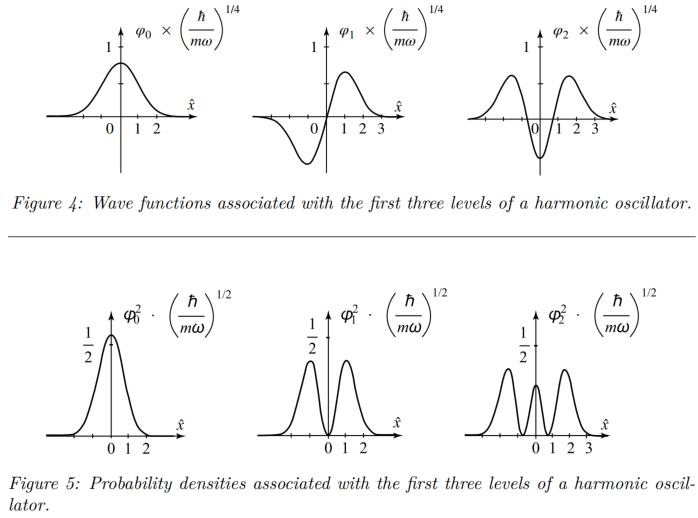
\includegraphics[width=.7\columnwidth]{PartOne/ChapterThree/excitedstatesqho.png}
\end{figure}


